\documentclass[11pt,a4paper]{article}
\usepackage[margin=0.88in]{geometry}
\usepackage[T1]{fontenc}
\usepackage[utf8]{inputenc}
\usepackage{lmodern}
\usepackage{microtype}
\usepackage{graphicx}
\usepackage{booktabs,tabularx,longtable,array}
\usepackage{amsmath,amssymb,mathtools}
\usepackage{float,subcaption}
\usepackage{xcolor}
\usepackage{hyperref}
\usepackage{fancyhdr}
\usepackage{enumitem}
\usepackage{placeins}
\graphicspath{{figures/}}
\definecolor{navy}{HTML}{17394D}
\definecolor{linkblue}{HTML}{1B6486}
\hypersetup{colorlinks=true,linkcolor=navy,urlcolor=linkblue,citecolor=linkblue,pdftitle={MAGFiLO V25: Developmental History, Failure Analysis, and Quality-Aware Solar Filament Instance Segmentation}}
\pagestyle{fancy}\fancyhf{}\lhead{MAGFiLO: End-to-End Development and V25 Evidence}\rhead{Extended technical manuscript}\cfoot{\thepage}\setlength{\headheight}{15pt}
\setlength{\parskip}{0.4em}\setlength{\parindent}{0em}
\newcommand{\PQ}{\mathrm{PQ}}\newcommand{\SQ}{\mathrm{SQ}}\newcommand{\RQ}{\mathrm{RQ}}
\newcommand{\RLE}{\mathrm{RLE}}\newcommand{\Halpha}{H$\alpha$}
\newcommand{\sourcefig}[1]{\textit{Source: #1.}}
\title{\vspace{-1.2cm}\textcolor{navy}{\Large From Semantic Masks to Quality-Aware Filament Instances:}\\[0.25em]
\textbf{An End-to-End Experimental Chronicle, Failure Analysis, and Frozen-Model Evaluation for the 2026 MAGFiLO Solar Filament Challenge}}
\author{Lighittha Pappusamy Rathika \and Prithivraj Selvakumar\\[0.4em]
\small Vellore Institute of Technology, Chennai, India\\
\small \texttt{ligpersonalmail@gmail.com} \quad \texttt{theprithivrajs@gmail.com}}
\date{Research archive prepared 2 November 2026\\\small Companion to the four-page Solar Filament Segmentation Challenge 2026 technical report}
\begin{document}
\maketitle
\begin{abstract}
Accurate delineation of solar filaments from 2048$\times$2048 Global Oscillation Network Group (GONG) H$\alpha$ images requires more than binary foreground prediction: models must recover separate structures without spurious fragments, duplications, or over-merging. This extended manuscript documents the complete observed evolution of a competition entry, from early semantic and compact-detector experiments at approximately 0.31--0.34 public Panoptic Quality (PQ), through negative investigations involving native crops, ridge classifiers, graph-based fragment repair, and clean-slate architecture searches, to a frozen quality-aware multiscale V25 pipeline associated with a user-confirmed rounded Kaggle public score of \textbf{0.39}. The scored artifact comprises 1,093 compressed-RLE filament instances and is retained under its exact SHA-256 fingerprint. The selected model combines two solar-adapted YOLO11m-seg detectors (full-disk global context and overlapping native-image windows), a learned 69-feature candidate-quality ensemble, and selective prompt-conditioned mask refinement. On 51 historically reused audit scenes spanning 46 acquisition days, the reconstructed pipeline obtains local pooled instance PQ of \textbf{0.45888} (SQ 0.67991, RQ 0.67492); frozen-component removals reduce PQ by 0.00990 for quality selection and by 0.01199 for mask refinement. A three-seed quality-estimator refit identifies detector support and H$\alpha$ appearance as consequential feature families. Further V28/V29 novel-instance recovery tests yield only +0.00032 and +0.00080 local audit PQ, respectively, and are not promoted over the proven public submission. We include timeline provenance, negative results, full method definitions, fixed-checkpoint ablations, descriptive day-cluster bootstrap intervals, filament-size stratification, expert disagreement, genuine observational overlays, and reproducibility requirements. \textbf{No independent-test performance, official-evaluator parity, or final competition placement is claimed.}
\end{abstract}
\tableofcontents
\newpage

\section{Problem, stakes, and definition of success}
Solar filaments are dark, elongated structures apparent in chromospheric H$\alpha$ imagery, closely associated with magnetic organization and potentially eruptive events. The MAGFiLO dataset supplies annotated filament instances, including polygonal masks, and constitutes a benchmark for scene-scale segmentation \cite{magfilo}. The 2026 challenge supplies 707 labeled competition-training images and 180 unlabeled competition-test images, both with 2048$\times$2048 full-disk observations \cite{challenge}. The distinction between the competition subset and the larger published MAGFiLO v1.0 collection is important: this work trains on the \emph{competition-permitted} annotations, not on external annotated test counterparts.

The unit of prediction is an \emph{individual filament instance}. A single foreground probability map can look visually plausible while losing separate objects, joining neighbors, or splitting long strands. Evaluation therefore uses Panoptic Quality (PQ), with instance matching based on overlap and recognition penalties, rather than relying on pixel-level foreground Dice alone \cite{kirillov}. The organizer also evaluates engineering quality, documentation, computational cost, and the morphology of predicted masks \cite{challenge}.

Our practical goals evolved over the project. First, establish a legitimate repeatable trained-model baseline rather than rely on opaque precomputed masks. Second, explain when finer native resolution actually helps instance recognition. Third, produce a stable set of masks with a learned assessment of whether each prediction deserves inclusion. Fourth, freeze the exact publicly scored submission and run genuine component-level experiments without retuning a historical test result. Finally, document failed hypotheses alongside successes, rather than presenting a falsely monotonic development story.

\paragraph{Evidence hierarchy.} Throughout, we distinguish \textbf{(P)} a rounded Kaggle public score recorded in experiment notebooks or confirmed by the user; \textbf{(L)} a score calculated on a specified, labeled local sample; \textbf{(H)} a method or training attempt documented in a source notebook without confirmed comparative score; and \textbf{(A)} an ablation carried out on the same historical audit scenes. The public 0.39 is a statement about the exact scored file, not about arbitrary regenerated outputs.

\section{Data organization, scoring, and reproducibility boundaries}
\subsection{Observed images, annotations, and scene identity}
Each image is treated as a 2048$\times$2048 grayscale H$\alpha$ observation. The training annotation JSON contains potentially multiple expert versions for a single physical scene. To avoid treating these versions as independent acquisitions, physical scenes are grouped by image stem; scene dates are taken from the first eight filename digits. Each available annotation polygon is rasterized as a separate instance; annotations are not concatenated into one indistinguishable foreground for the instance objective. Standard COCO run-length encoding is used for efficient mask interchange.

The original V20 detector training placed 104 acquisition-day-grouped images outside its 603-image training population. Subsequent experiments repeatedly revisited those 104 images, including repeated recipe selection and error analysis. The final evidence notebook subdivides them into 53 \emph{historical calibration} and 51 \emph{historical audit} scenes (46 audit acquisition days). The separation is useful for training a new quality-model ablation and comparing variants on different days, but the audit is \textbf{not a newly untouched test set}. The actual unlabeled competition test contains 180 images.

\subsection{PQ and related metrics}
Let $G$ be the set of expert filament masks and $P$ the predicted instances for a scene. Hungarian assignment is applied to the IoU matrix. A proposed pair is considered a match if $\operatorname{IoU}(p,g)>0.5$; unmatched predictions and references count as false positives and false negatives. For paired set $TP$, the local evaluator computes
\begin{equation}
\PQ=\frac{\sum_{(p,g)\in TP}\operatorname{IoU}(p,g)}{|TP|+\tfrac{1}{2}|FP|+\tfrac{1}{2}|FN|}=\SQ\cdot\RQ,
\end{equation}
where $\SQ$ is the average IoU of matched objects and $\RQ=|TP|/(|TP|+\tfrac12|FP|+\tfrac12|FN|)$. The historical implementation pools these numerator and denominator contributions across available expert versions; foreground Dice is computed independently from the union masks. \textbf{The organizer's reference implementation may differ in edge cases or aggregation.} Official parity has not been demonstrated by this archive.

\subsection{Frozen scored public artifact}
The original scored V25 file is \texttt{V25\_REAL\_REFINE\_PLUS\_QUALITY.csv}, preserved in the repository as \texttt{V25\_EXACT\_PUBLIC\_039.csv}. It has 1,093 rows (one per predicted instance), with columns \texttt{filament\_id} and \texttt{segmentation\_rle}. Its full SHA-256 is
\begin{quote}\small\ttfamily ac470fbfa0e2ca5f2d8a654d6c6bbaf549dd8980d040963ed8ba4821dc9ac329\end{quote}
The user-confirmed rounded Kaggle public score is \textbf{0.39}. This is the best historically confirmed public result in the attached evidence. In the final component-ablation run, the original CSV was verified but the optional all-test-image reconstruction check was \emph{disabled}; thus exact regeneration parity of the full 180-image inference procedure remains unproven.

\section{Development history: what we tried, why, and what happened}
\subsection{A non-monotonic public-score trajectory}
Figure~\ref{fig:progress} records representative public milestones from notebook narratives. They are \emph{distinct submitted recipes}, not epochs of one model and not a controlled same-split test. The observed trajectory is explicitly non-monotonic: research steps that looked promising in local validation sometimes produced worse public performance. The early scoring-method revision is another reason to avoid extrapolating between old public reports without qualification.

\begin{figure}[H]\centering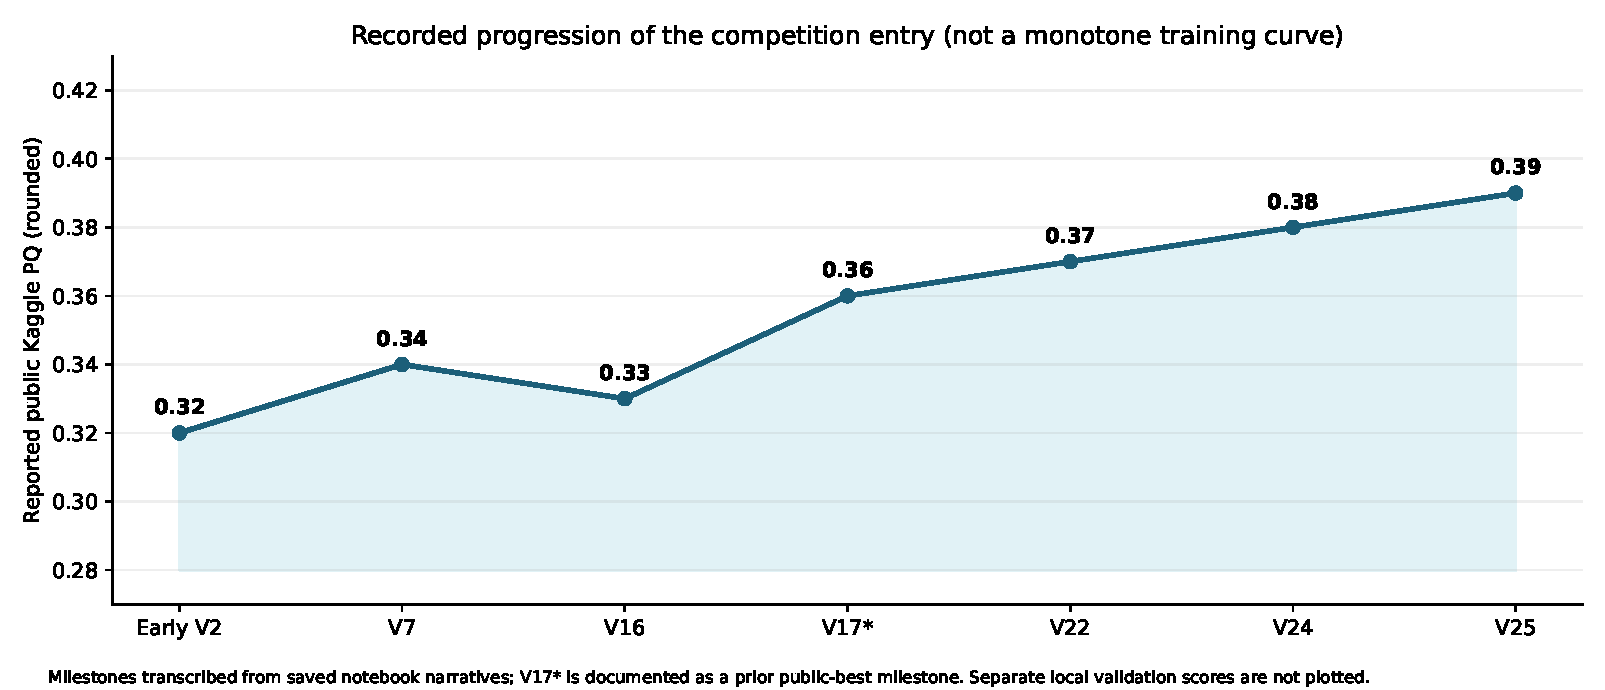
\includegraphics[width=.96\textwidth]{Fig00_development_milestones.pdf}
\caption{Select rounded public-score milestones recorded during development. V17 is included as a documented previous-best milestone, not a fully preserved scored CSV in the current release. Historical local validation numbers are deliberately excluded.}\label{fig:progress}\end{figure}

\begin{longtable}{p{.115\textwidth}p{.28\textwidth}p{.49\textwidth}}
\caption{Research chronology: experiments, outcomes, and evidence strength. Negative runs are included; a blank public score does not imply zero performance.}\label{tab:chronology}\\
\toprule \textbf{Phase} & \textbf{Change and hypothesis} & \textbf{Observed outcome, failure, and takeaway} \\ \midrule\endfirsthead
\toprule \textbf{Phase} & \textbf{Change and hypothesis} & \textbf{Observed outcome, failure, and takeaway} \\ \midrule\endhead
V1--V4 & Semantic segmentation, detector/refiner baselines, instance-aware training, confidence policies. & Early public results around 0.28--0.32 (P, notebook narratives). A locally optimistic 0.4135 from a 20-image tuning subset did not predict public PQ. Semantic pixel accuracy alone did not resolve instance identity.\\
V5--V6 & Restore actual learned checkpoints; compare legitimate public-reference architecture and local PQ instead of opaque mask files. & Emphasized model provenance and avoiding unverified precomputed submissions (H). Compact detector output and scale loss remained concerns; confirmed public recipes around 0.31.\\
V7--V7.1 & Native-resolution tiled inference and overlap arbitration using a CPU-friendly YOLO11n-seg model. & A V7-derived user-reported 0.34 public reference became the protected control (P). Native tiling improved the candidate search but required careful seam rejection; an output was only promoted if actually scored.\\
V8--V8.1 & Fine-tune a tile specialist with native crops, then evaluate a global/tile hybrid. & Thirteen training epochs produced checkpoint weights, but evaluation initially failed because cached window tuples were serialized as JSON lists and rejected during equality checks (H). This was a reproducibility bug, not negative model evidence.\\
V9 & Multi-scale dark-ridge / topology classifier (LightGBM) trained on permitted masks. & The reported V9 public output was 0.31, associated with selection of the older V4 fallback (P). A newly trained pixel learner did not automatically improve the instance-level end result.\\
V10--V11 & Learned candidate quality, consensus, and a fragment-graph merge classifier. & V10 exported 0.33 in one recorded attempt while the V7 0.34 reference remained better (P). Inaccurate baseline reconstruction and risk of merging unrelated filaments complicated causal interpretation (H).\\
V12--V15 & Exact historical submission recovery, OOF delta-PQ actions, risk-aware deletion and fragment rescue. & One apparently large +0.0488 grouped OOF gain was later traced to comparison against an \emph{incorrectly reconstructed} reference, not the proven 0.34 file (H). Hash-locking the true CSV prevented false improvement claims.\\
V16 & Clean-slate training: ResUNet, multiple FPN semantic models, YOLO11s/m segmentation. & Best local YOLO11m PQ 0.38993 on a 97-scene V16 tune population, but public result about 0.33 (L/P). Some semantic models had higher matched overlap but worse detection precision, reinforcing the instance-level objective.\\
V17--V20 & Higher-resolution windows, trained solar-specialized YOLO11m detectors, acquisition-day grouping. & Historical public-best milestone about 0.36 before later ranking recipes (P, notebook narratives). Native/global detector complementary outputs proved useful, but one cannot transfer local V16 scores across differently grouped splits.\\
V22--V23 & Freeze two-source 1792-global + 1280-window mask generation; select candidates with occupancy and seam policy. & V22 alternative 2 was documented at public 0.37 (P). Two-source fusion stabilized the high-recall candidate bank.\\
V24 & Prompt-conditioned V24 refinement and 15-feature quality estimation. & V24 quality-0.25 configuration documented at public 0.38 (P). Candidate filtering reduced false positives; reliance on saved weights and reproducible feature order became important.\\
V25 & Curve evidence, 69-feature ranker, real-error mask refiner and restricted final decoder. & Exact 1,093-row scored CSV documented at public \textbf{0.39} (P); this is the frozen competition submission retained for all later comparisons. On the historical audit the reconstructed method obtains PQ 0.45888 (A).\\
V26 & Retrain on real detector errors and learn a counterfactual refinement selector. & New hypotheses and checkpoints were developed (H); no independently verified public score higher than 0.39 is established in the supplied archive.\\
V27 & Instance-query FilamentFormer-Lite with Hungarian assignment, centerline/boundary supervision. & A genuine separate architecture was trained and archived (H), but its own run report retained 0.39 as the best confirmed public outcome. Successful training alone was not evidence of public improvement.\\
V28 & New high-resolution solar-pretrained detector and quality-gated novel-instance fusion. & Of 502 candidate-training examples, 32 were qualifying new-instance positives. Best conservative fusion gained only +0.000323 \emph{local} PQ; HR detector alone scored 0.321324 local audit, far below V25 control (L). No promotion.\\
V29 & Novelty-credit regressors, fragment-pair proposals, rank ensembles. & Of 363 candidate-training examples, 61 were qualifying positives. Mean-ranked fusion gained +0.000798 local audit PQ; most ranking alternatives left V25 unchanged or worsened it (L). No promotion.\\
V30 & Further paper and historical comparison work referenced in logs. & Full independent executed V30 result with new confirmed public improvement is \emph{not available} in this archive; we neither attribute a numeric gain nor introduce a fictional model.\\
\bottomrule
\end{longtable}

\subsection{Failure categories and what was learned}
\textbf{Wrong objective:} semantic foreground Dice and patch detector mAP can improve while object-level PQ remains flat or falls. V16's semantic ensembles and the V8 validation mAP are not interchangeable with leaderboard instance PQ.

\textbf{Resolution alone is insufficient:} viewing 2048-pixel images through overly small network inputs suppresses fine barbs. Native windows recover some details but also increase duplicate detections, sever objects at seams, and change the domain seen by a detector. The V28 HR model underperformed on the reused audit despite its additional training.

\textbf{Unstable or incorrect baselines:} reconstruction-dependent tests can yield illusory deltas. V12--V15 exposed this problem, motivating the immutable original CSV fingerprint and independent method names.

\textbf{False positives from plausible proposals:} novel candidate masks can resemble filaments but are costly under PQ when they fail one-to-one instance matching. V28 and V29 quantify this directly: many candidate masks are not genuinely uncovered true objects.

\textbf{Infrastructure and serialization failures:} the V8 tuple/list cache mismatch blocked evaluation. Such a failure must be recorded as a software error, not silently scored as a failed model.

\textbf{Repeated reuse of the same audit:} each additional attempt reduces its credibility as a fresh measure of generalization. We disclose the entire development process so the final descriptive intervals are not mistaken for confirmatory confidence limits.

\begin{figure}[H]\centering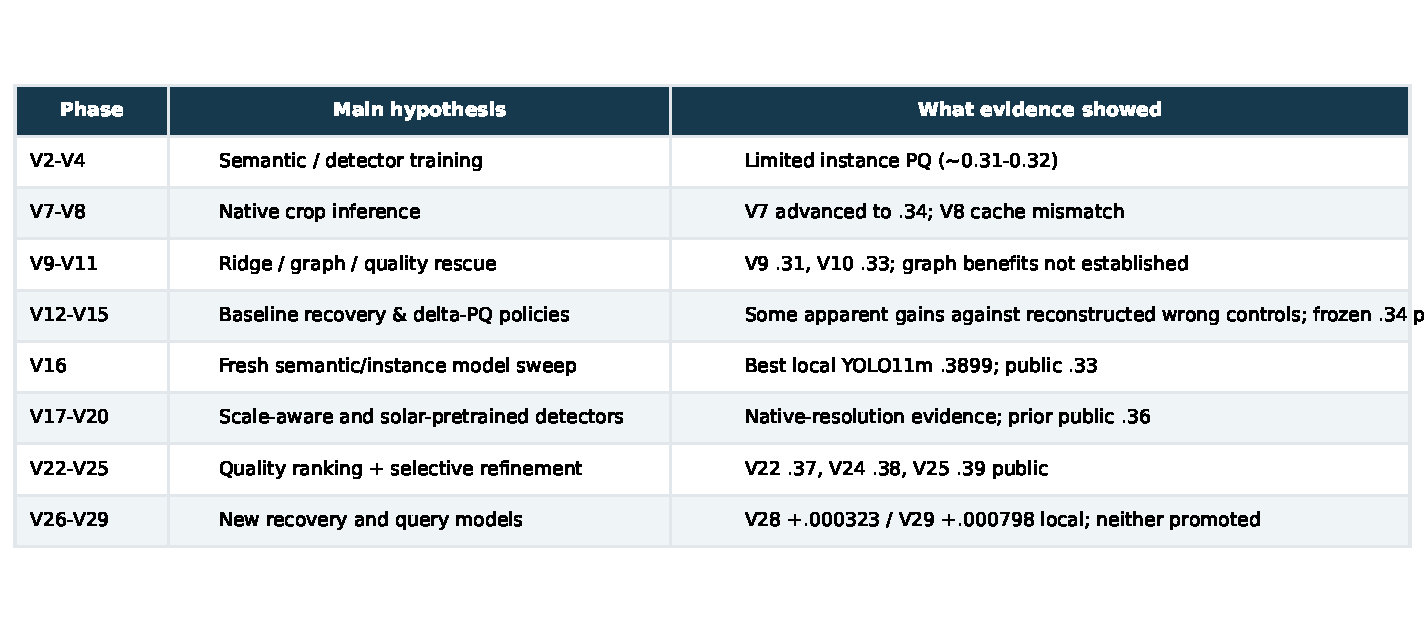
\includegraphics[width=.98\textwidth]{Fig00_failures_matrix.pdf}
\caption{Summary of eight distinct development regimes and the failure/success mode supported by source notebooks. This is a narrative synthesis, not a statistical model comparison.}\end{figure}

\section{Final frozen V25 architecture and inference mechanics}
\subsection{Source observations and global/native detectors}
The final detector stage is based on two \emph{separately trained solar-adapted} YOLO11m-seg checkpoints \cite{ultralytics}: \texttt{portable\_global\_m\_best.pt} and \texttt{portable\_native\_m\_best.pt}, each with 22,359,987 parameters. The global detector consumes the full 2048-square image resized by the network to 1792 pixels. The native detector operates on four overlapping 1280$\times$1280 source-space crops, each fed to the segmentation network at 1024 pixels. Crops begin at coordinates $\{0,768\}$ along each axis. The prediction mask is mapped from network to crop resolution and inserted at its original global coordinates. The raw confidence threshold is 0.08, raw IoU NMS 0.72, \texttt{agnostic\_nms=True}, \texttt{retina\_masks=True}, and \texttt{max\_det=120}. The two branches offer complementary global context and fine detail.

\subsection{Geometric filtering, seam guard, and overlap arbitration}
For the selected V22/V25 detector recipe, global candidates must meet confidence 0.24 and native-window candidates 0.42. Masks under 200 source pixels are removed. Native masks touching interior crop borders within a 10-pixel tolerance are discarded by the seam guard. A bonus of 0.08 is added to native confidence for sorting, not interpreted as calibrated probability. Sorted candidate RLEs are rejected as duplicates if their mask IoU with any prior source mask exceeds 0.50. For each surviving mask, pixels already claimed by earlier accepted masks are excluded; at least 45\% of the original candidate area must remain free, and at least 200 free pixels must survive. This produces nonoverlapping instances.

\begin{figure}[H]\centering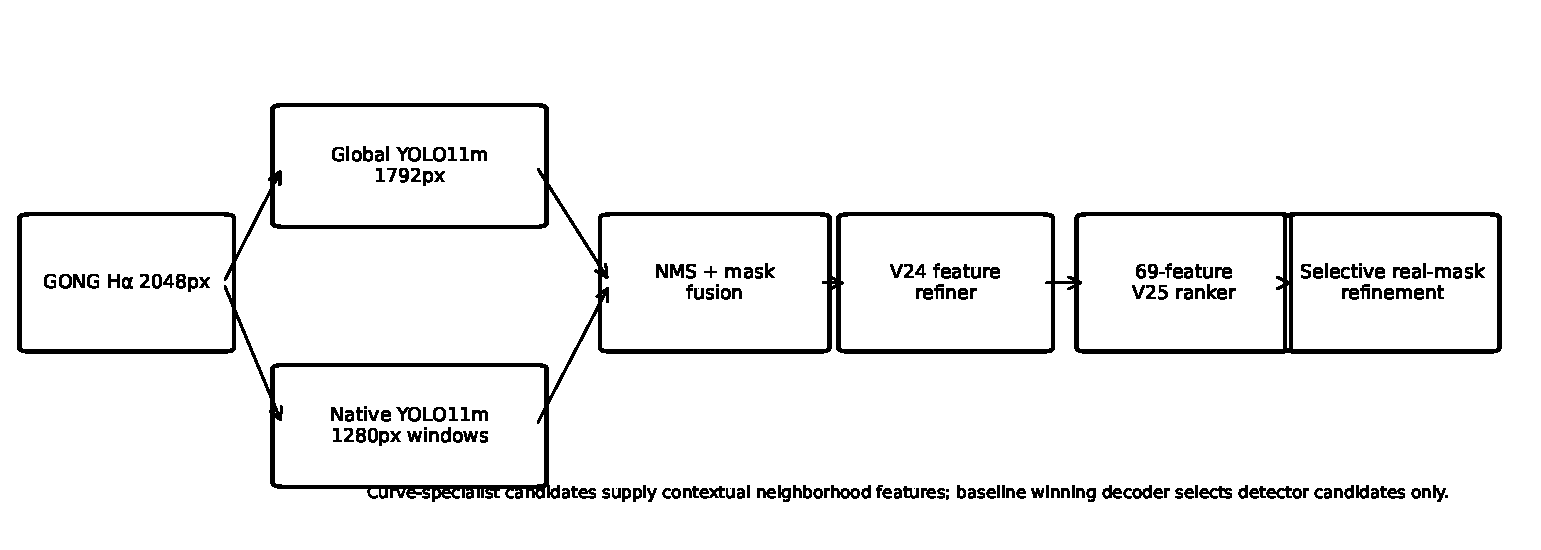
\includegraphics[width=.96\textwidth]{Fig00_frozen_V25_pipeline_schematic.pdf}
\caption{Schematic of the frozen 0.39-entry V25 reconstruction. The curve specialist is an auxiliary candidate/context source; \emph{the publicly selected decoder keeps detector-origin candidates}, not automatically all curve predictions.}\label{fig:architecture}\end{figure}

\subsection{V24 learned refinement context}
A prompt-conditioned encoder-decoder, initialized with a four-channel ResNet18-style input stem, ingests grayscale, contrast-limited adaptive histogram equalization, a binary prompt mask, and an edge-magnitude channel. A 320$\times$320 crop around a proposed filament is passed to its trained encoder-decoder; refined masks are accepted only within area-ratio and original-prompt-IoU gates. The frozen V24 feature set includes 15 quantities: candidate score and geometry, location, global/native support, local pixel contrast, and refinement-change measurements. Its historical 0.25 threshold controls a V24 baseline; it is \emph{not} identical to the final V25 ranker.

\subsection{Curve specialist and 69-feature quality representation}
The curve specialist is a compact two-channel-to-three-channel U-Net with about 0.99M parameters. It processes nine overlapping 768-pixel source windows after resizing to 512 pixels. Its outputs include foreground, centerline, and an auxiliary channel; connected components may be split conservatively where distinct centerline seeds are detected. Candidate area and confidence gates, rejection of internal crop-edge fragments, and mask-IoU deduplication limit excessive proposals. The historical V25 final decoder did not directly accept curve-origin instances; candidate and context computations can still use their presence. The later experiment explicitly adding curve-origin masks is treated as a changed decoder, not evidence for the scored configuration.

The V25 quality learner consumes a fixed \textbf{69-feature ordered vector}, composed of the V24 feature columns and additional morphology/appearance/support/context variables. The principal feature groups are: (i) detector support (confidence, source agreement, source ranking); (ii) H$\alpha$ appearance (inside/ring intensity, gradient, contrast, entropy); (iii) topology and geometry (skeleton length, endpoints, branch points, thickness, elongation, solidity, area); and (iv) neighborhood position (distance and overlap with nearby proposals, solar-limb distance and center). It loads an ensemble from \texttt{SOLAR\_V25\_EXTENDED\_QUALITY.joblib}. The stored cutoff is 0.38 and the feature \emph{order} is checked against the serialized checkpoint.

\subsection{Selective real-mask refinement and final RLE}
Only detector-origin predictions assigned quality at least 0.38 are selected. Those with predicted quality at least 0.50 are additionally processed by \texttt{SOLAR\_V25\_REAL\_REFINER\_BEST.pt}, a 13.75M-parameter prompt-conditioned model trained with real detection errors. A proposed refinement is rejected when it departs excessively from the original prompt mask; source-frame RLEs are then occupancy-clipped again. Each final instance becomes a unique \texttt{filament\_id} followed by compressed mask counts. This selective policy, rather than unconditional refinement or indiscriminate candidate addition, identifies the publicly scored V25 method.

\section{Final same-scene frozen-component ablations}
\subsection{Audit setup and key comparisons}
The executed final evidence notebook reconstructs all 12 frozen-method variants on the same 104 historical scenes and reports the 51-scene audit separately from the 53-scene calibration subset. The weights are not retrained in these component-removal experiments. Table~\ref{tab:ablation} includes scores from the actual exported CSV, including both the core component removals and two contextual policy variants. \emph{Only the original preserved test CSV has a confirmed public 0.39 score.}

\begin{table}[H]\centering\small
\caption{Frozen-method component ablations on the 51 historically reused audit scenes, 46 acquisition days. All scores are \emph{local PQ}, not Kaggle public results. ``No quality ranker'' additionally changes which masks pass the conditional-refinement gate.}\label{tab:ablation}
\begin{tabular}{lrrr}\toprule Configuration & PQ & SQ & $\Delta\PQ$\\\midrule
Always refine accepted & 0.459313 & 0.680546 & +0.000433\\
\textbf{Full V25 reconstructed} & \textbf{0.458880} & 0.679905 & ---\\
No curve context & 0.458397 & 0.679190 & -0.000483\\
Lower quality cutoff 0.30 & 0.457717 & 0.676836 & -0.001163\\
Include curve candidates & 0.456719 & 0.680066 & -0.002161\\
Higher quality cutoff 0.46 & 0.455476 & 0.682043 & -0.003404\\
No quality ranker & 0.448975 & 0.676552 & -0.009905\\
No real-mask refiner & 0.446886 & 0.670329 & -0.011994\\
V24 quality gate & 0.444146 & 0.668354 & -0.014734\\
Two-detector fusion only & 0.436862 & 0.665936 & -0.022018\\
Global detector only & 0.433451 & 0.668868 & -0.025429\\
Native detector only & 0.363140 & 0.677861 & -0.095740\\
\bottomrule\end{tabular}
\end{table}

The full reconstructed method yields $TP=409$, $FP=164$, and $FN=230$ under pooled expert-version accounting (SQ 0.679905, RQ 0.674917, mean foreground Dice 0.616415). The global-only source is stronger than native-only in this audit; the native source nevertheless improves the fusion when supported by the global branch. The two-detector-only configuration has 431 TP but 244 FP: recognition precision is the major issue. The quality ranker reduces false positives and selects fewer objects while retaining sufficient true detections. Real-mask refinement improves both the matched-IoU numerator and, through acceptance and clipping, the matched-instance counts in this particular comparison.

\begin{figure}[H]\centering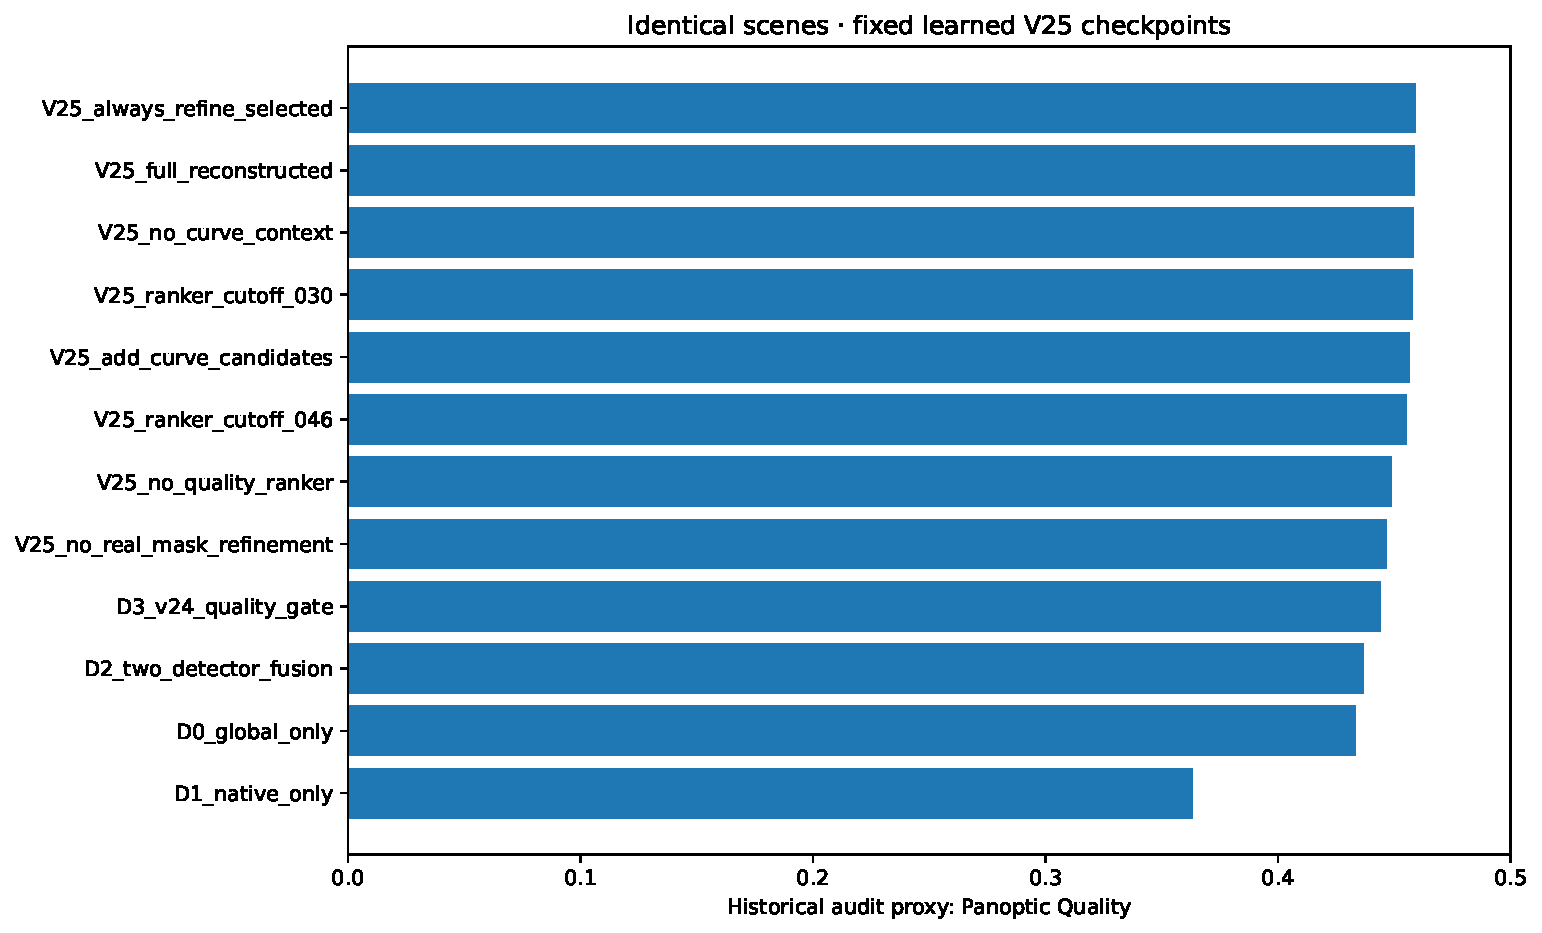
\includegraphics[width=.96\textwidth]{Fig01_V25_component_ablation_PQ.pdf}
\caption{All twelve frozen-component configurations from the final V25 evidence run. These measures share an evaluation population and scoring implementation; values do not represent separate public submissions.}\end{figure}

\subsection{Descriptive day-cluster paired uncertainty}
Paired day-cluster bootstrap resampling (2,000 replicates) preserves method pairing within each of the 46 audit days and recomputes pooled PQ. For removing the real-mask refiner, the mean bootstrap difference from full is approximately $-0.0120$ (95\% percentile interval $[-0.01826,-0.00655]$). Removing quality ranking gives approximately $-0.00984$ (interval $[-0.02016,-0.00021]$). Merely adding curve candidates gives approximately $-0.00218$ (interval $[-0.00458,-0.00037]$), illustrating that increasing candidate count can worsen object-level performance. Always refining selected masks yields a tiny positive difference of $+0.00043$ (interval $[-0.00014,+0.00099]$), insufficient to justify a strong claim. These intervals describe sensitivity within a \emph{historically explored} audit, not a prospective inference population.

\begin{figure}[H]\centering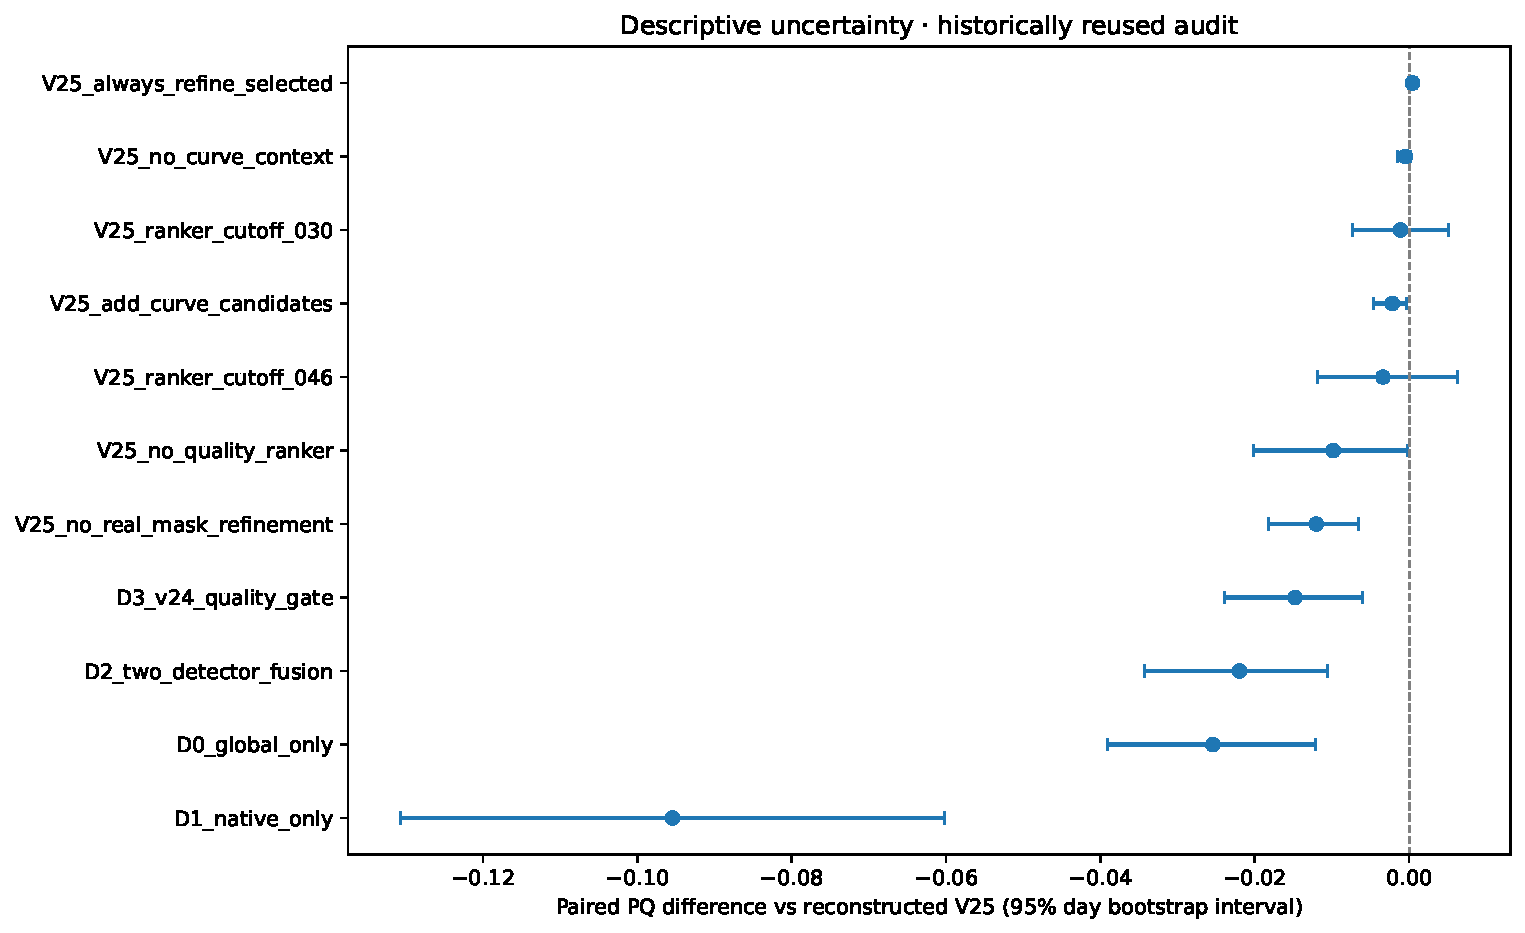
\includegraphics[width=.97\textwidth]{Fig02_component_PQ_deltas_CI.pdf}
\caption{Actual paired day-bootstrap local-PQ differences against full V25. The zero reference and intervals support conservative interpretation of both failures and apparently positive changes.}\label{fig:bootstrap}\end{figure}

\section{Ranker retraining, calibration, and morphology}
\subsection{Three-seed feature-family refits}
Unlike zeroing a trained model's features at inference (an out-of-distribution intervention), the feature-family study fits new estimators on the historical 53-scene calibration subset and assesses them on the 51-scene audit subset, with random seeds 2026, 2037 and 2048. Each fit uses a histogram gradient-boosting classifier and an ExtraTrees classifier. The frozen V25 ranker remains unchanged. All candidate features are derived from images and predictions, never hidden test labels.

\begin{table}[H]\centering
\caption{Three-seed mean historical-audit PQ for quality-ranker feature-family retraining. Variance reflects ranker refitting only, not independently trained detector backbones.}\label{tab:features}
\begin{tabular}{lrr}\toprule Feature design & Mean PQ & SD\\\midrule
All 69 features & 0.458923 & 0.000938\\
Without detector-support cues & 0.444527 & 0.000534\\
Without H$\alpha$ appearance cues & 0.448959 & 0.000504\\
Without shape/topology cues & 0.457419 & 0.000932\\
Without neighborhood/context cues & 0.458944 & 0.000505\\
\bottomrule\end{tabular}
\end{table}

The ranking evidence suggests that cross-detector support and local image appearance are valuable for deciding whether an instance should be retained. Topological descriptors show a weaker measured contribution in this small historical audit, and removing neighborhood descriptors changes the mean score negligibly. This does \emph{not} prove physical solar topology is unimportant; it only describes the contribution of this particular feature encoding within this model and dataset.

\begin{figure}[H]\centering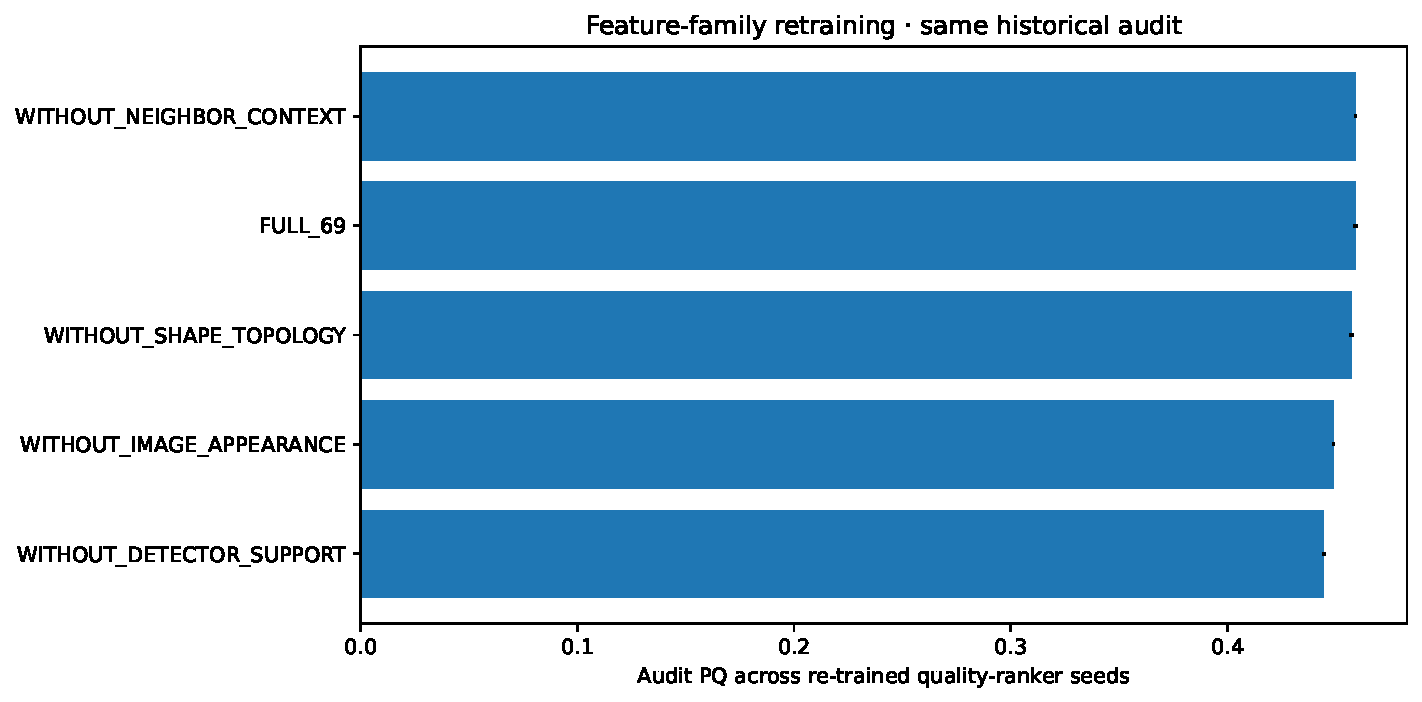
\includegraphics[width=.92\textwidth]{Fig05_retrained_ranker_feature_ablation.pdf}
\caption{Mean and cross-seed variability of retrained feature-family rankers.}\end{figure}

\subsection{Reliability and selective processing}
Predicted quality probabilities are compared with observed expert-agreement positives in ten coarse bins, using the held historical audit and the first refit seed. The exported reliability table contains 763 candidate estimates. Several middle-to-high probability bins deviate from the $y=x$ line, demonstrating imperfect calibration; these outputs should be interpreted as selection scores, not formally calibrated posterior probabilities. The quality cutoff of 0.38 remains locked to the historical chosen method.

\begin{figure}[H]\centering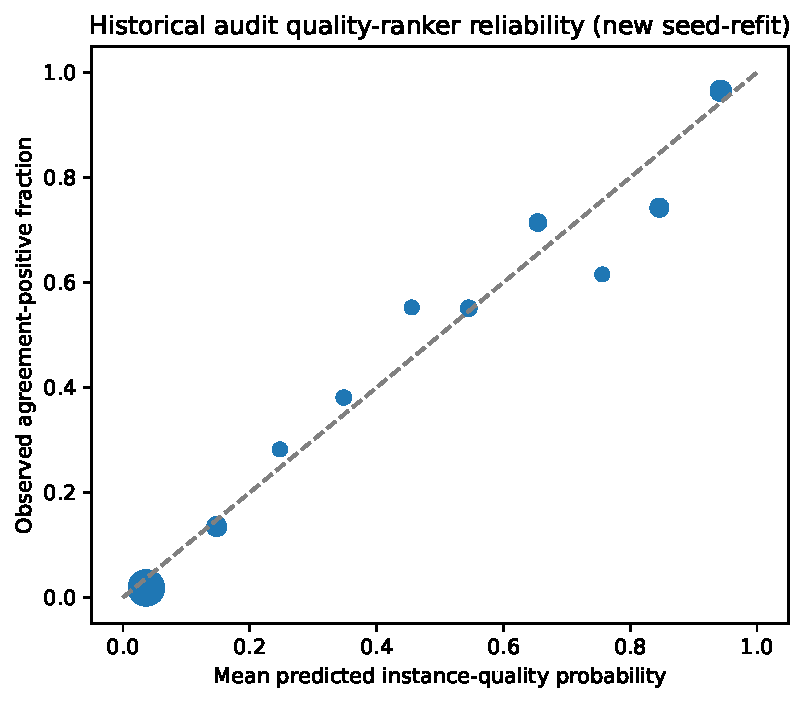
\includegraphics[width=.74\textwidth]{Fig06_ranker_reliability.pdf}
\caption{Reliability analysis for one seed-refit quality estimator, not a universal calibration certificate.}\end{figure}

\subsection{Filament size, separation, and inter-annotator differences}
Among the audit's expert-instance records, the model recalls 167 of 294 tiny objects ($<1000$ pixels; 0.568), 201 of 284 small objects (1,000--5,000 pixels; 0.708), and 40 of 57 medium objects (5,000--20,000 pixels; 0.702). Only four objects exceeded 20,000 pixels, so the corresponding 0.25 recall is too sparsely sampled for broad inference. The tiny-object deficit is an actionable weakness; increasing the number of small masks without a trustworthy acceptance policy can still reduce PQ.

Thirty-eight expert-annotation pairs are available across the audit scenes. Their mean pairwise PQ is 0.4004; this reflects annotation disagreements as captured by the local matching protocol, not a theorem that model PQ cannot exceed 0.4004. Likewise, one-to-many and many-to-one overlaps are logged using an exploratory overlap threshold of 0.1; these indicate possible fragmentation and merging but have not been manually confirmed as distinct physical failure events.

\begin{figure}[H]\centering
\begin{subfigure}{.49\textwidth}\centering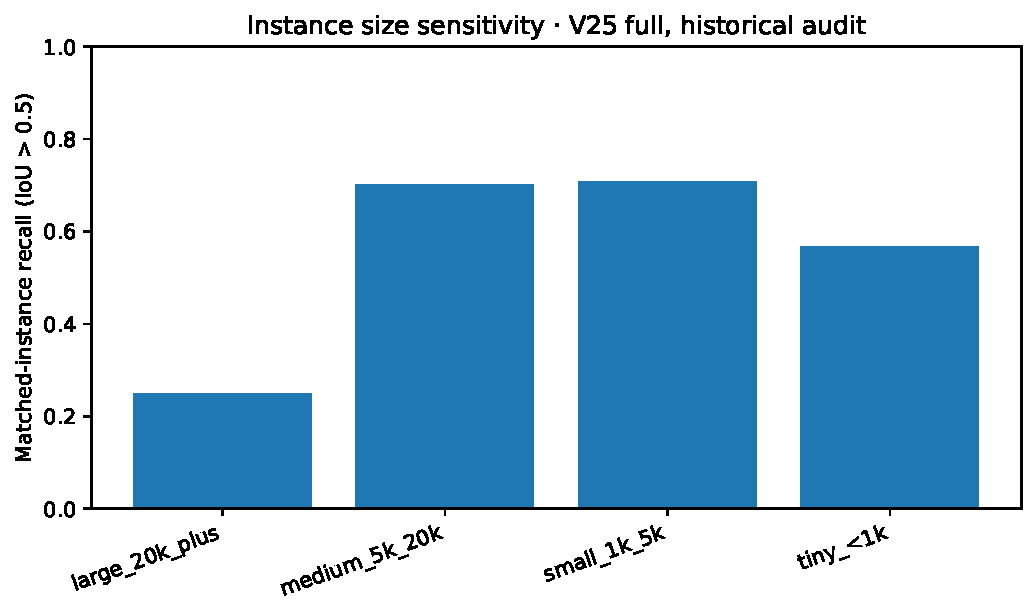
\includegraphics[width=\linewidth]{Fig03_V25_instance_size_recall.pdf}\caption{Instance-size recall.}\end{subfigure}\hfill
\begin{subfigure}{.49\textwidth}\centering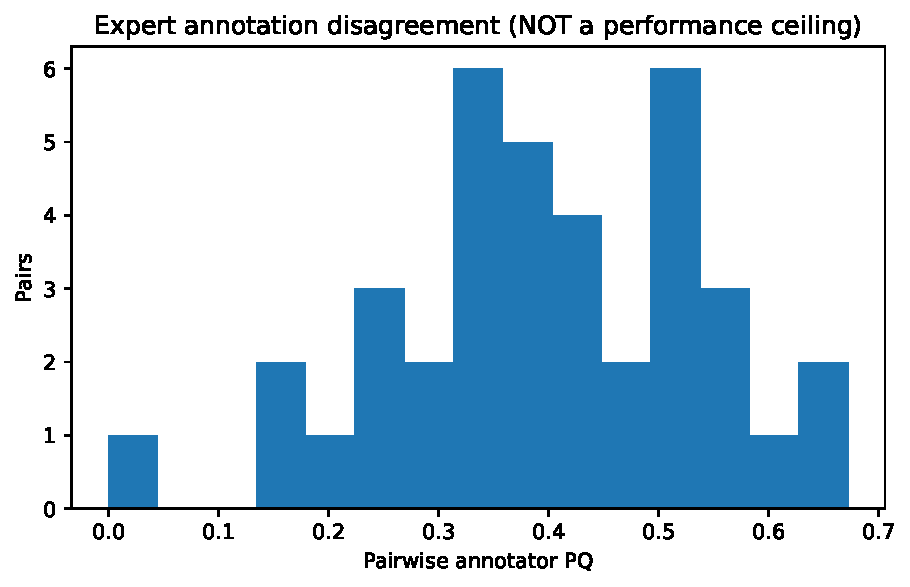
\includegraphics[width=\linewidth]{Fig04_expert_agreement.pdf}\caption{Expert-pair PQ variation.}\end{subfigure}
\caption{Observed structural and labeling challenges in the final historical audit.}\label{fig:morph}\end{figure}

\section{Qualitative observations and failure cases}
Eight case panels in the final evidence ZIP show actual labeled H$\alpha$ observations, not synthesized data. Each panel compares detector-only output, output without real-mask refinement, and the reconstructed full V25 output. Green denotes overlap between predicted and expert-foreground pixels, yellow indicates expert foreground not predicted, and red indicates excess predicted foreground. These colors describe \emph{pixelwise} overlap, not formally matched TP/FP/FN instances. Case scenes were selected among low and high per-scene local-PQ examples; selection was made after inspecting historical local outcomes, so the panels illustrate failure modes but are not representative random samples.

\begin{figure}[H]\centering
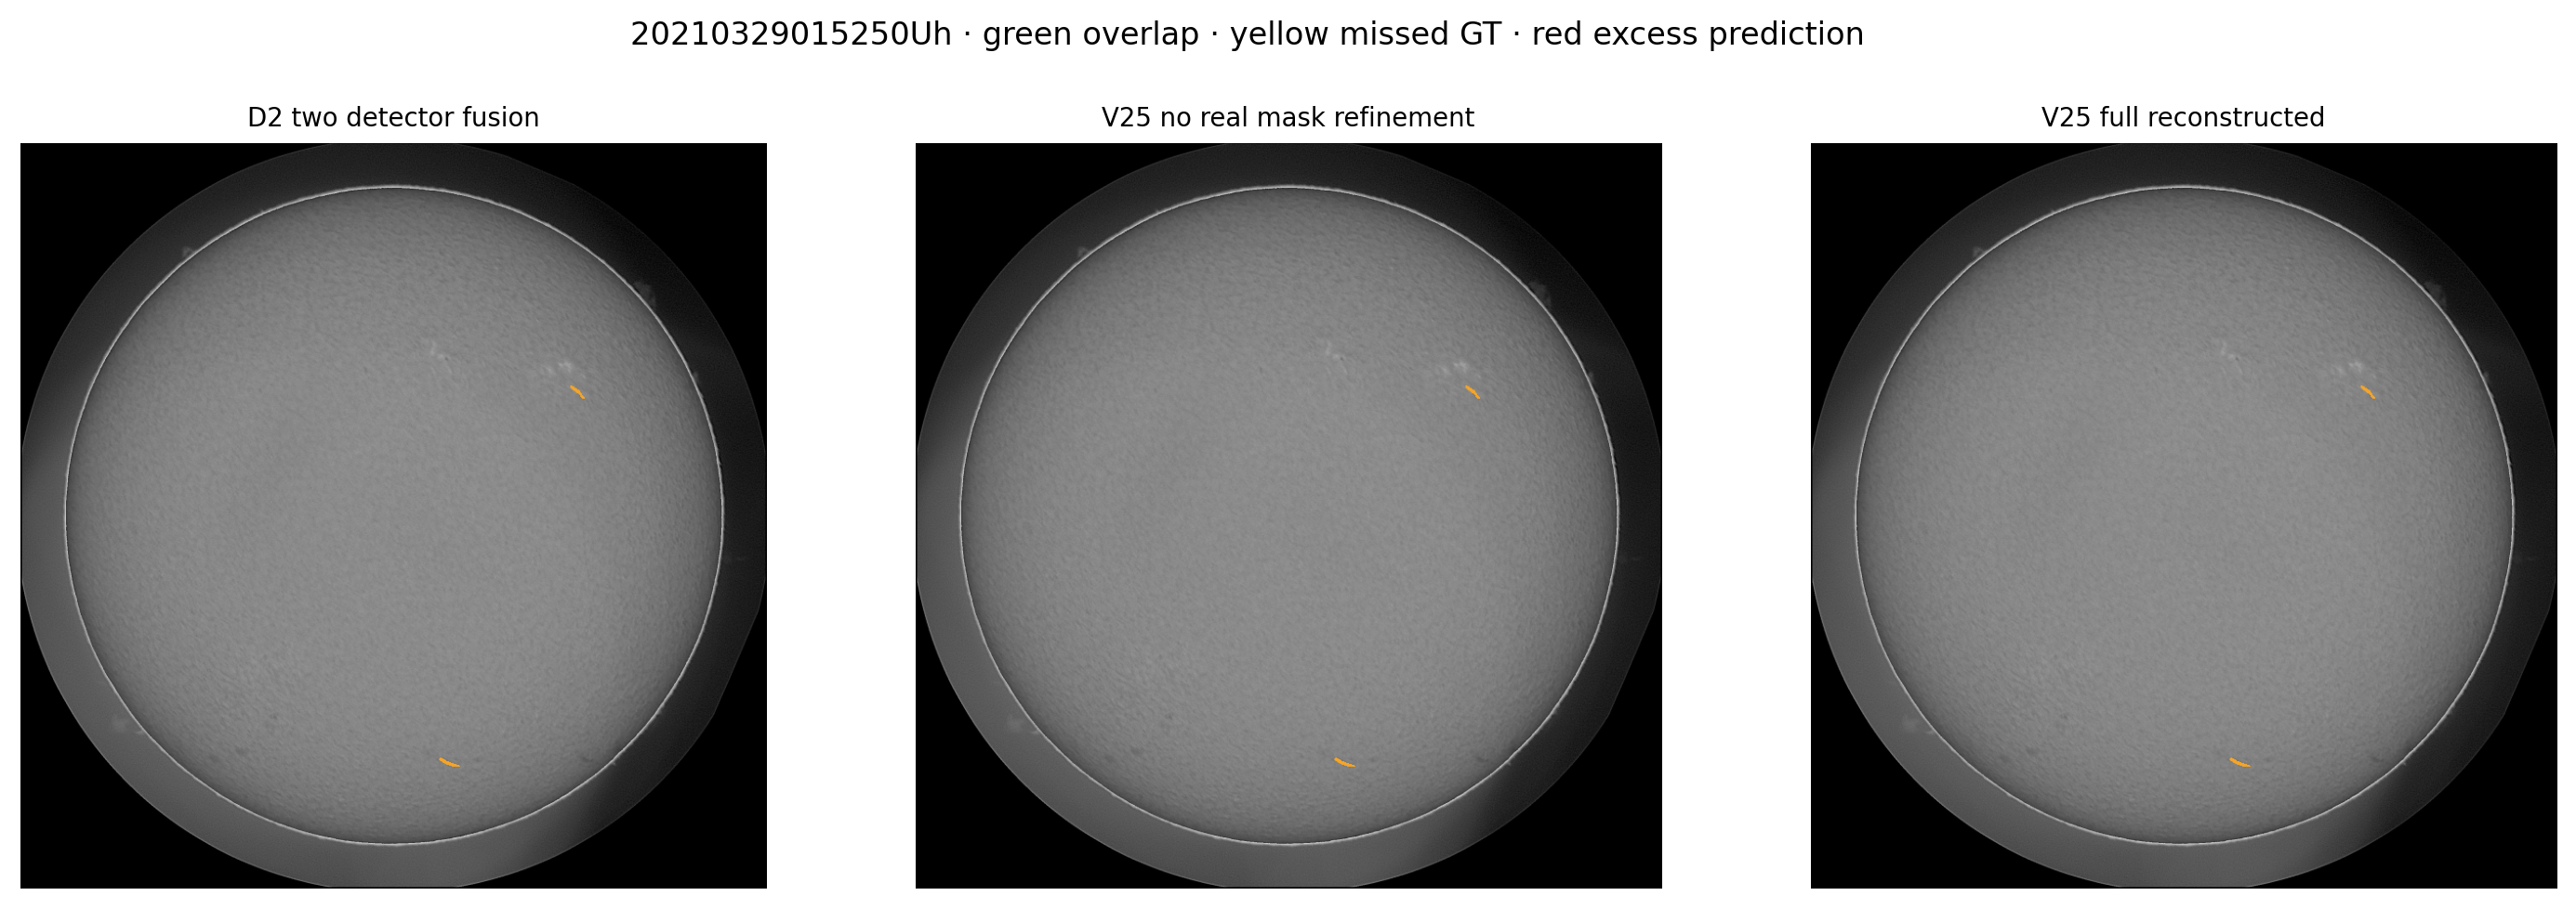
\includegraphics[width=.97\textwidth]{Fig07_case_01_20210329015250Uh.png}
\caption{An actual low-scoring audit case from the supplied evidence. Compare detection-only, no-refinement, and full predictions against a single expert version.}\end{figure}
\begin{figure}[H]\centering
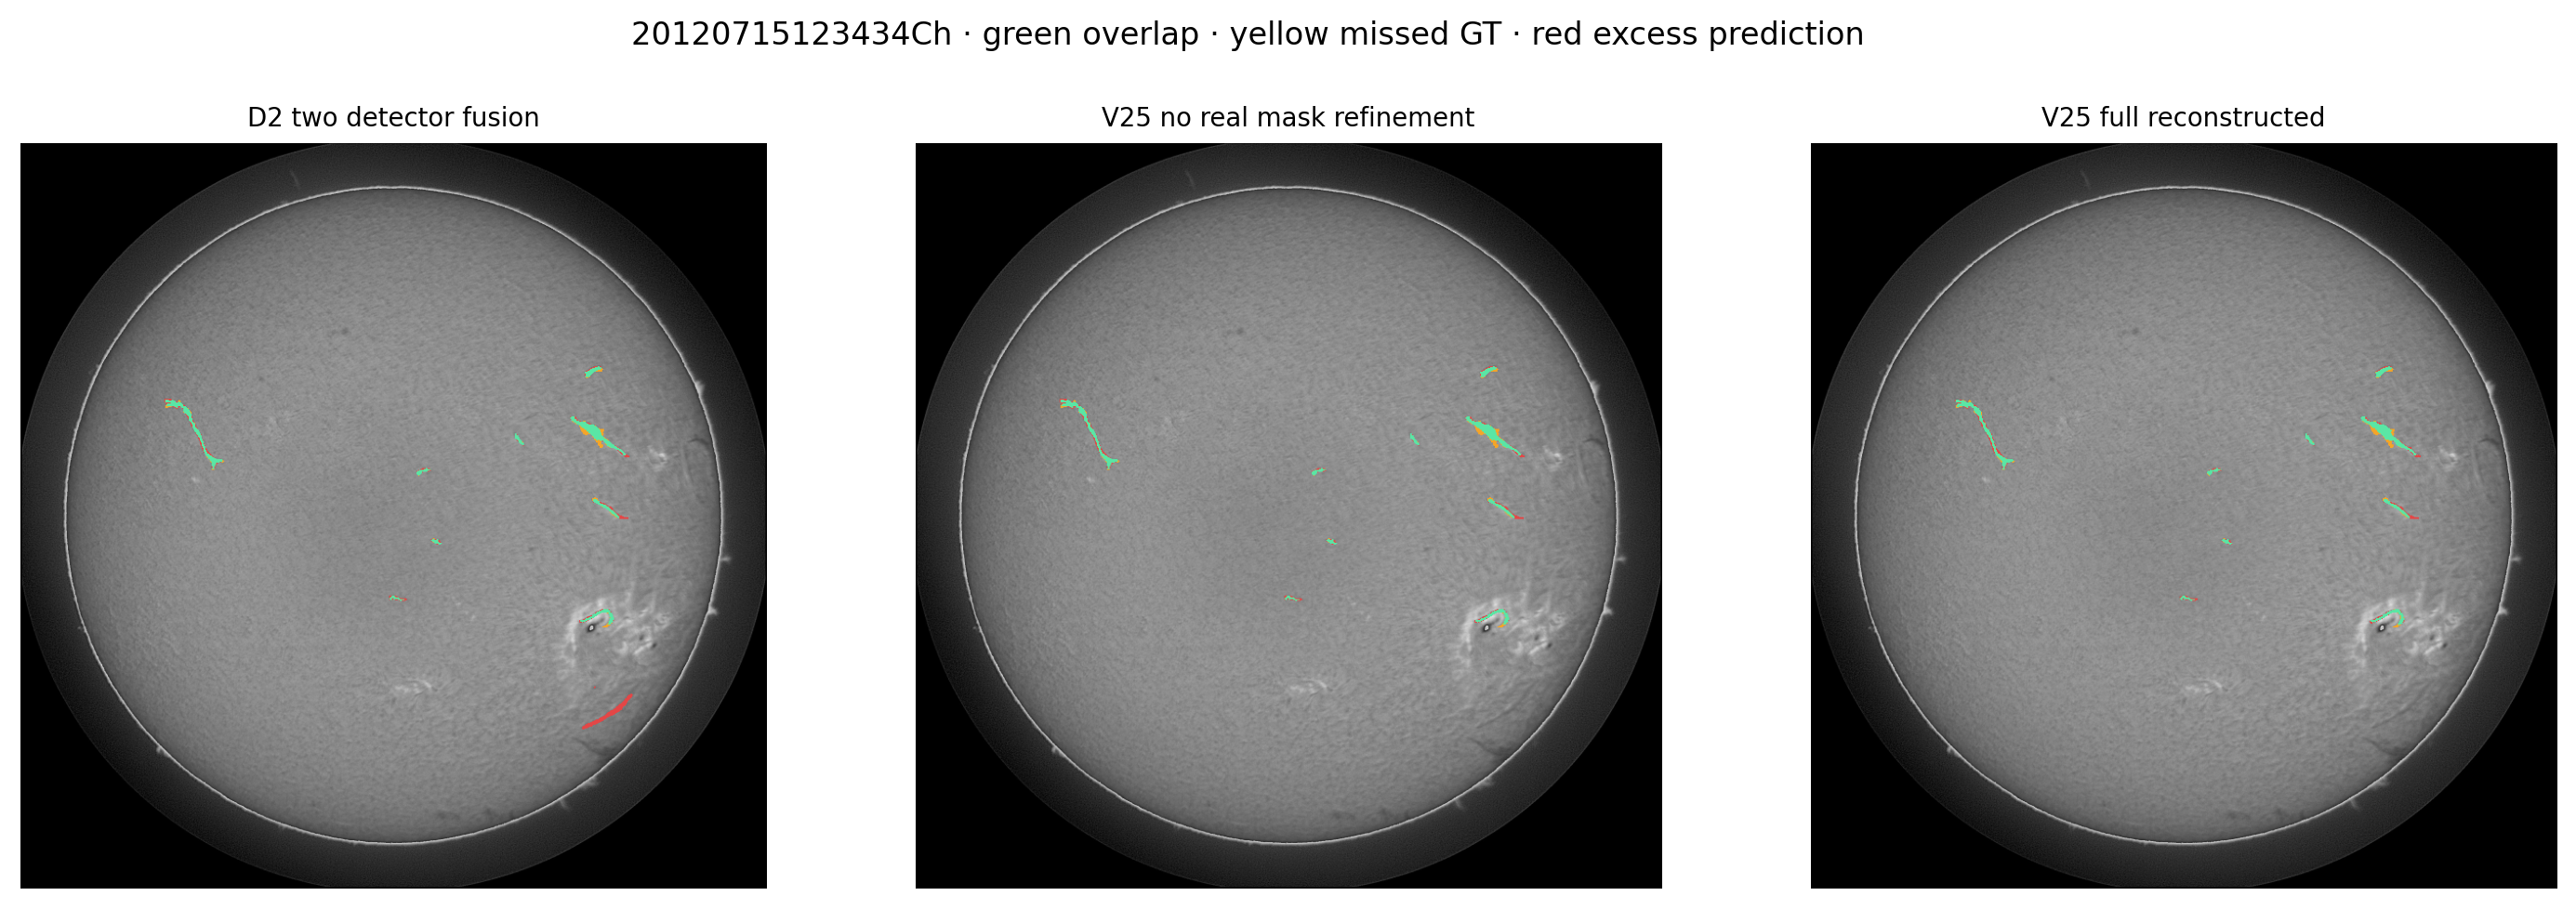
\includegraphics[width=.97\textwidth]{Fig07_case_06_20120715123434Ch.png}
\caption{A second observation from the saved final-V25 case-selection set; line morphology and predicted/expert disagreement remain visibly important.}\end{figure}

The common qualitative risks are: faint dark features mistaken for filaments, false positives near active regions, incomplete thin barbs, split detections at tile borders, and competing masks of overlapping structures. The evidence suggests rejecting untrustworthy candidates often matters as much as making a foreground mask look smoother. It also supports retaining honest examples of the model's limits rather than using only successful visualizations.

\section{V26--V29: why additional models did not replace V25}
Once the V25 file achieved the user-confirmed 0.39 public score, the later experiments used it as a protected control rather than overwrite it with any newly trained network. V26 trained a refinement/counterfactual selector on real prediction errors. V27 introduced learned instance queries and Hungarian assignment with filament-specific geometric supervision. These are substantive experimental branches but, in the supplied evidence, lack a separately confirmed superior public submission. The V28/V29 runs include completed local-audit numerical comparisons and a candidate-yield analysis.

\begin{table}[H]\centering\small
\caption{Later-run local-audit results. Numbers originate from uploaded execution-log transcriptions; they are \emph{not} freshly independently recomputed from matching per-scene archives here. All local V25 reference rows have PQ 0.458880.}\label{tab:later}
\begin{tabular}{lrrr}\toprule V28/V29 variant & Local PQ & $\Delta\PQ$ & Local FP\\\midrule
V28 high-res detector alone & 0.321324 & -0.137556 & 227\\
V28 raw confidence fusion & 0.457866 & -0.001014 & 180\\
V28 conservative fusion & 0.459203 & +0.000323 & 165\\
V28 learned-novel fusion & 0.458880 & 0.000000 & 164\\
V29 novelty mean rank & 0.459678 & +0.000798 & 164\\
V29 pessimistic/rank/agreement variants & 0.458880 & 0.000000 & 164\\
V29 V24/V25 blended ranking & 0.441855 & -0.017025 & 109\\
\bottomrule\end{tabular}
\end{table}

The V28 candidate training population contained 502 possible additions, with just 32 classified as genuinely useful uncovered instances (6.37\%). The V29 development set contained 363 candidate examples, with 61 qualifying positives (16.80\%). Recovering positives is necessary but not sufficient for better PQ: each new output also increases the denominator unless it becomes a legitimate one-to-one match. The conservative V28 fusion improvement has a historically reported interval $[-0.001055,+0.002157]$, and the V29 mean-ranked improvement has $[0,+0.002915]$ (the latter includes zero). Both were below the prespecified audit-gain cutoff 0.004 and did not meet the bootstrap support threshold 0.90. V25 stayed the selected public control.

\begin{figure}[H]\centering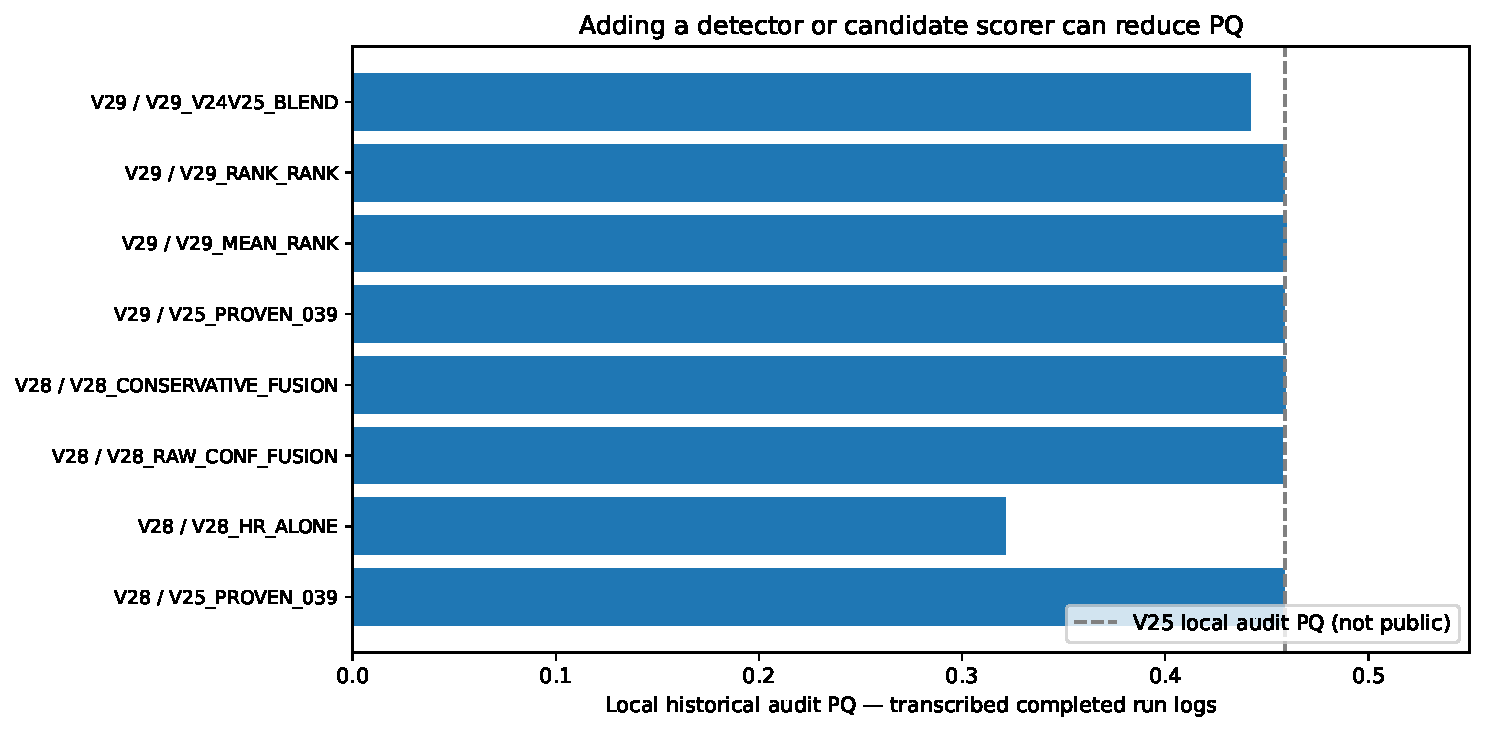
\includegraphics[width=.94\textwidth]{Fig12_v28_v29_completed_log_audit_comparison.pdf}
\caption{V28/V29 historical local-audit PQ, transcribed from the uploaded completed logs; do not interpret as public Kaggle scores or direct independent-test improvement.}\end{figure}
\begin{figure}[H]\centering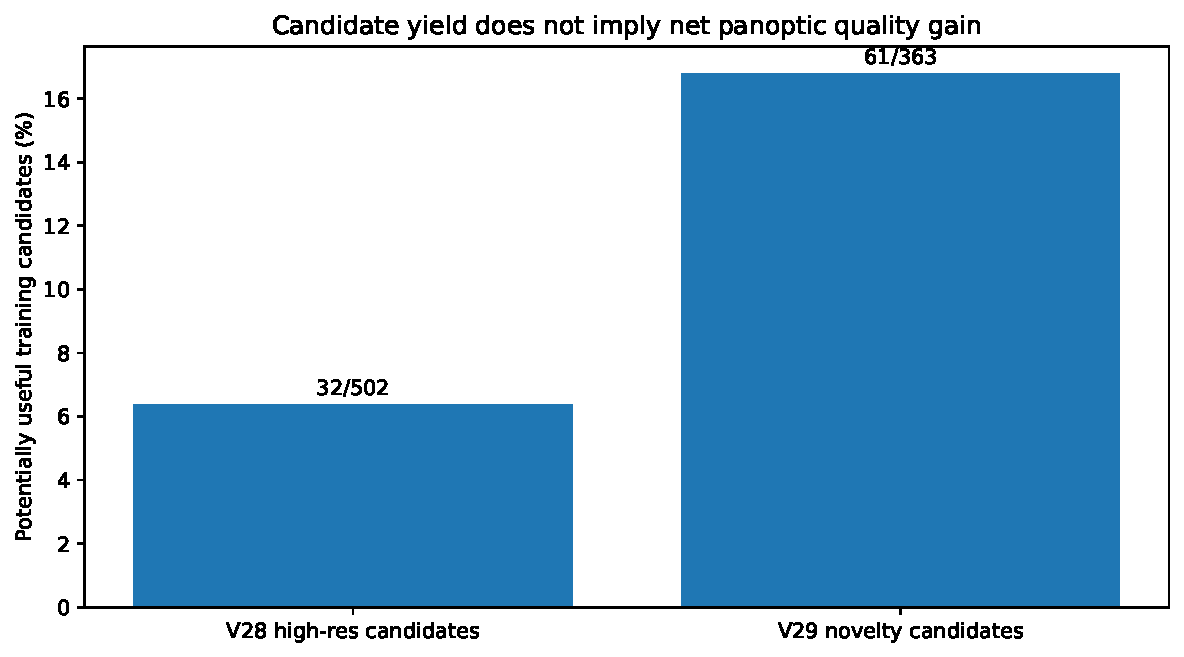
\includegraphics[width=.88\textwidth]{Fig11_qualifying_novelty_candidates_log.pdf}
\caption{Qualified positive candidate share in V28 and V29. Candidate mining differs between runs, so percentages are not a controlled isolated comparison of models.}\end{figure}

\section{Compute, model inventory, and archival integrity}
The frozen models have the following parameter counts: each YOLO11m detector 22,359,987, the V24 prompt refiner 13,752,897, the V25 real-mask refiner 13,752,897, and the compact V25 curve network 990,451. The two quality-model checkpoints are serialized scikit-learn objects. The executed final study reported a peak PyTorch CUDA allocated memory of 0.91 GiB and a mean of 13.89 seconds per scene across \emph{all variants plus shared caches}; these are not an independent single-configuration latency benchmark and should not be advertised as deployment inference throughput. The historical study also contains separate detector latency measurements from an earlier protocol, whose population and scope must be kept distinct.

Seven exact checkpoint fingerprints are in \texttt{models/checkpoint\_manifest.json}. SHA-256 verification is a precondition for calling an attached model the archived original. The reproducibility notebook is configured to use the official competition images, the genuine checkpoint files, and the original scored CSV; it produces a \emph{new} reconstructed CSV and an all-180-scene original-versus-regenerated overlap report. An exact publicly scored file is preserved even if regeneration changes mask ordering or numeric outputs. Original checkpoints were not supplied among the artifacts available for this research-release build; they are not falsely included in the downloadable GitHub ZIP. A team preparing the final public repository must add all seven weight/model assets or working, accessible Git-LFS links before claiming complete inference reproduction.

\section{Discussion: contribution and appropriately limited conclusion}
The development history supports a specific engineering-scientific result: a global/native ensemble with mask occupancy arbitration supplies candidate recall; a learned, shape- and image-aware quality model reduces unnecessary instances; and selective prompt-conditioned refinement improves the geometry and reliability of chosen objects. On the historically reused V25 audit, each of the latter two stages has measurable influence, while direct inclusion of curve proposals and aggressive new-instance recovery do not clearly help. This is a more defensible technical claim than asserting every new architecture improves PQ.

The chronological negative experiments are integral to interpretation. The V8 cache problem was software, the V12--V15 apparent gains were undermined by reference inconsistency, V16 showed that strong local single-model results can fail to transfer to public evaluation, and V28/V29 showed that novel instance generation remains dominated by a cost-of-false-positive trade-off. None of these observations implies an algorithmic impossibility; each suggests a higher-quality next experiment with stronger controls.

The largest limitations are: (1) repeatedly consulted local audit data, not a pristine prospective test; (2) absence of independent acquisition/observatory generalization evaluation; (3) no complete multi-seed retraining of original detector/refiner backbones; (4) no verified parity between the historical local PQ proxy and the competition's official evaluator; (5) no completed exact all-180-scene re-inference equivalence test; and (6) source notebooks and a scored CSV without the trained checkpoint bytes in this attached archive. Accordingly, we regard this document as a \textbf{detailed competition research record and extended technical manuscript}, not as proof of a new state-of-the-art generalization claim or a competition win.

\section{Competition submission versus archival paper}
The organizer requests a separate four-page technical report in the provided ACM-style Overleaf template, one publicly accessible code repository with \texttt{requirements.txt} and weights, a notebook reproducing the final prediction pipeline, and a Google Form submission \cite{challenge}. The present extended document is supplementary research detail and would not replace the required concise report. A separate peer-reviewed workshop paper would have its own submission gate, format, and review decisions. The package contains \texttt{competition\_4page.pdf} and source beside this longer research history; neither document is automatically accepted for publication merely by submitting a Kaggle entry.

\section*{Acknowledgments and data credit}
The competition organizers, the National Solar Observatory, and the GONG instrumentation/data teams are acknowledged. The accompanying challenge-format report retains the organizer-provided formal NSF/NSO/GONG acknowledgment text. The MAGFiLO dataset and competition organizers are cited explicitly \cite{magfilo,challenge}. Author contributions, exact current affiliation, and any institutional approvals should be confirmed by the submitting team before upload.

\begin{thebibliography}{9}\setlength{\itemsep}{2pt}
\bibitem{magfilo} A. Ahmadzadeh, R. Adhyapak, K. Chaurasiya, et al. ``A dataset of manually annotated filaments from H-alpha observations.'' \emph{Scientific Data}, vol. 11, article 1031, 2024. \href{https://doi.org/10.1038/s41597-024-03876-y}{doi:10.1038/s41597-024-03876-y}.
\bibitem{challenge} A. Ahmadzadeh, D. J. Kempton, Q. Li, and A. A. Pevtsov. ``Solar Filament Segmentation Challenge 2026.'' Kaggle, 2026. \url{https://www.kaggle.com/competitions/filament-segmentation-2026}.
\bibitem{kirillov} A. Kirillov, K. He, R. Girshick, C. Rother, and P. Doll\'ar. ``Panoptic Segmentation.'' In \emph{Proceedings of the IEEE/CVF Conference on Computer Vision and Pattern Recognition}, 2019. \href{https://doi.org/10.1109/CVPR.2019.00963}{doi:10.1109/CVPR.2019.00963}.
\bibitem{unet} O. Ronneberger, P. Fischer, and T. Brox. ``U-Net: Convolutional Networks for Biomedical Image Segmentation.'' In \emph{MICCAI}, 2015. \href{https://doi.org/10.1007/978-3-319-24574-4_28}{doi:10.1007/978-3-319-24574-4\_28}.
\bibitem{maskrcnn} K. He, G. Gkioxari, P. Doll\'ar, and R. Girshick. ``Mask R-CNN.'' In \emph{Proceedings of the IEEE International Conference on Computer Vision}, 2017. \href{https://doi.org/10.1109/ICCV.2017.322}{doi:10.1109/ICCV.2017.322}.
\bibitem{ultralytics} Ultralytics. ``Ultralytics YOLO11 Documentation.'' \url{https://docs.ultralytics.com/models/yolo11/}. Software documentation, accessed 2026.
\end{thebibliography}

\appendix
\section{Supplementary gallery: eight real V25 audit cases}
The following appendix preserves the additional source panels. Their selection mixes lower- and higher-local-PQ observations and is intended for diagnostic visualization. Each source image comes from the permitted labeled competition train set. The complete per-scene and per-expert tables are present in the accompanying code release, with original filenames and hashes.
\newcommand{\casefigure}[2]{\begin{figure}[H]\centering\includegraphics[width=.98\textwidth]{#1}\caption{#2}\end{figure}}
\casefigure{Fig07_case_02_20210626060050Uh.png}{V25 selected case 02: diagnostic image/label comparison across three true model configurations.}
\casefigure{Fig07_case_03_20181024232430Lh.png}{V25 selected case 03: visual evidence of remaining filament-background ambiguity.}
\casefigure{Fig07_case_04_20170801164710Mh.png}{V25 selected case 04: reconstructed instance and foreground overlap.}
\casefigure{Fig07_case_05_20131206084114Th.png}{V25 selected case 05: historical audit observation.}
\casefigure{Fig07_case_07_20110902073614Th.png}{V25 selected case 07: historically high/low comparison sample.}
\casefigure{Fig07_case_08_20161210133714Th.png}{V25 selected case 08: historical audit observation.}

\section{Supplementary historical detector analysis}
These plots come from a \emph{separate} V20--V30 evidence-lab execution on 105 labeled scenes (98 acquisition days), not the 51-scene V25 component-audit protocol. The best reported detector-only configuration in that earlier analysis reached local PQ 0.3804 compared with its own fixed detector reference of 0.2526. The figures illustrate scale sensitivity and failure morphology but their numbers must not be substituted into Table~\ref{tab:ablation} or used as the public 0.39 score.
\casefigure{Fig05_selected_area_recall.pdf}{Earlier detector study: object-size recall under a different evaluation population.}
\casefigure{Fig10_fragmentation_diagnostic.pdf}{Earlier detector study: exploratory fragmentation/overlap diagnostics.}
\casefigure{Fig07_learning_00.pdf}{Training-history figure preserved from the earlier detector evidence archive; not evidence of V25 quality-ranker convergence.}

\section{Artifact and claim checklist}
\begin{enumerate}[leftmargin=*]
\item \textbf{Exact public result:} scored 1,093-row V25 CSV hash verified; public value 0.39 is user-confirmed, rounded, and applies only to these bytes.
\item \textbf{Same-scene local result:} 51 historically reused audit scenes, 46 days; 12 frozen variants; separate calibration of 53 scenes.
\item \textbf{Seeds:} three quality-classifier refits; not three independently trained YOLO or U-Net systems.
\item \textbf{Refinement:} 0.01199 local PQ reduction when removed; descriptive intervals conditional on reused audit.
\item \textbf{Curve branch:} context removal negligible; inclusion of additional curve-origin detections reduces PQ in the reported audit.
\item \textbf{Negative branches:} V26--V29 were researched, but no new confirmed public improvement over the protected V25 entry is supported.
\item \textbf{Weights:} model hashes recorded; actual checkpoint bytes must be added to public repository before a fully reproducible competition submission.
\item \textbf{Official parity:} not established; verify against organizer's self-evaluation notebook.
\item \textbf{Submission status:} no Google Form submission, GitHub publication, peer-review acceptance, or competition placement is asserted by this package.
\end{enumerate}
\end{document}
